%----------------------------------------------------------------------
% Introduction

\begingroup
\allowdisplaybreaks

\section{Introduction}

A key challenge for self-driving cars is autonomous navigation. Autonomous navigation fuses the inputs of multiple sensors to formulate a position, velocity, and attitude (PVA) solution for the vehicle of interest. Common navigation sensors include inertial measurement units (IMUs), global positioning system (GPS) receivers, odometers, magnetometers, radars, LiDAR, cameras, and many others. It is crucial to not only formulate a navigation solution but also to track the uncertainty of that solution, which can play an important role in decision-making and risk-assessment for autonomous self-driving vehicle applications.

IMUs generally contain three accelerometers and gyroscopes pointing in all three Cartesian axes which measure specific force and angular velocity respectively. These measurements are integrated to provide a PVA solution, but an IMU-only solution will drift away from truth unbounded due to the integration of sensor noise and other errors \cite{groves2013principles}. An inertial navigation system (INS) integrates the IMU measurements and then uses GPS to provide accurate measurements of position to fuse with the IMU solution typically via a Kalman filter thus combating any position error drift. This allows for long-term accurate navigation suitable for a self-driving car traveling long distances.

A driving need for navigation regarding self-driving cars is forming back-up modes of navigation when GPS signals are temporarily unavailable. This is especially important in urban environments where tall buildings and tunnels can cause signal blockages. Lack of GPS signals are problematic for an INS as its performance is dependent on receiving those signals, and the IMU-only solutions will drift away quickly from ground truth. Inertial-only navigation is suitable for short periods such as temporary GPS signal blockages, but the duration of a suitable inertial-only navigation is highly dependent on the quality of sensors contained within an IMU. This dilemma, among any others, motivates the need for rigorous IMU calibration and compensation.

One particular challenge with the use of commercial-grade or automotive-grade micro-electrical mechanical system (MEMS) inertial sensors is their sensitivity to temperature. Characterizing how common error sources such as bias, scale factors, and misalignments shift in response to temperature is a tough problem which requires hours of testing per unit and is often too burdensome for applications using automotive-grade devices. 

\subsection{Defining Sensor Error}

Accelerometers and gyroscopes are subject to a variety of error sources such as biases, scale factor imperfections, axis misalignments, noise, and many others. IMU calibration is the process of characterizing these error sources, while compensation is the process of correcting measurements in real-time to provide the most accurate and precise measurements possible. The better these error sources are characterized, the slower that the IMU-only navigation solution will drift away from truth. 

Inertial sensor calibration can be treated as an inverse problem. Consider an accelerometer as an example where the ideal forward model is quite straight forward; specific force in equals specific force out. Unfortunately in practice, we are not quite so lucky. Any error in the forward model is defined as

\begin{align*}
	\Delta f \defeq \tilde{f} - f
\end{align*}

where $\Delta f$ is the measurement error, $\tilde{f}$ is the specific force measured by the sensor which is subject to error, and $f$ is the true specific force acting on the accelerometer. The same applies to gyroscope measurements. 

\begin{align*}
	\Delta \omega \defeq \tilde{\omega} - \omega
\end{align*}

Inertial sensor errors $\Delta f$ and $\Delta \omega$ are subject to both deterministic and stochastic error and any number of contributing factors can make up these terms.

There are many procedures available to calibrate inertial sensors such as \cite{ImprovedIMUCalibrationProcedures} which require high-precision equipment to point and spin inertial sensors at known directions or quantities to separate measurement truth from measurement error.

\subsubsection{Basic IMU Error Sources and Error Models}

Consider an IMU which contains three accelerometers and three gyroscopes arranged to point in a standard Cartesian right-handed coordinate frame. A basic forward model framework appropriate for commercial- and automotive-grade inertial sensors is provided in \cite{groves2013principles}. 

\begin{align} \label{eq: compact IMU forward error model}
	\tilde{\bv{f}} &= \left[I + M_a\right] \bv{f} + \bv{b}_a + \bv{w}_a, \,\,\,\,\, \bv{w}_a \sim N\left(0,\,\sigma^2\right) \notag\\
	\\
	\tilde{\bv{\omega}} &= \left[I + M_g\right] \bv{\omega} + \bv{b}_g + \bv{w}_g \,\,\,\,\, \bv{w}_g \sim N\left(0,\,\sigma^2\right) \notag
\end{align}

In these models are bias terms $\bv{b}_a, \, \bv{b}_g \in \R^3$ for the accelerometers and gyroscopes respectively. In addition are the misalignment matrices $M_a, \, M_g \in \R^{3 \times 3}$, whose diagonal elements are scale factor error terms. The off-diagonal elements are misalignment terms which account for imperfections in the alignment of the sensing axes. All inertial sensors are also subject to noise, which is captured by terms $\bv{w}_a,\,\bv{w}_g$ which are additive zero-mean white Gaussian noise. Equation \ref{eq: expanded IMU forward error model} restates equation \ref{eq: compact IMU forward error model} in terms of all its various elements.

\begin{align} \label{eq: expanded IMU forward error model}
	\begin{bmatrix} \tilde{f}_x \\ \tilde{f}_y \\ \tilde{f}_z \end{bmatrix} &= \begin{bmatrix} 1 + s_{a,x} & m_{a,xy} & m_{a,xz} \\ m_{a,yx} & 1 + s_{a,y} & m_{a,yz} \\ m_{a,zx} & m_{a,zy} & 1 + s_{a,z} \end{bmatrix} \begin{bmatrix} f_x \\ f_y \\ f_z \end{bmatrix} + \begin{bmatrix} b_{a,x} \\ b_{a,y} \\ b_{a,z} \end{bmatrix} + \begin{bmatrix} w_{a,x} \\ w_{a,y} \\ w_{a,z} \end{bmatrix} \notag\\
	\\
	\begin{bmatrix} \tilde{\omega}_x \\ \tilde{\omega}_y \\ \tilde{\omega}_z \end{bmatrix} &= \begin{bmatrix} 1 + s_{g,x} & m_{g,xy} & m_{g,xz} \\ m_{g,yx} & 1 + s_{g,y} & m_{g,yz} \\ m_{g,zx} & m_{g,zy} & 1 + s_{g,z} \end{bmatrix} \begin{bmatrix} \omega_x \\ \omega_y \\ \omega_z \end{bmatrix} + \begin{bmatrix} b_{g,x} \\ b_{g,y} \\ b_{g,z} \end{bmatrix} + \begin{bmatrix} w_{g,x} \\ w_{g,y} \\ w_{g,z} \end{bmatrix} \notag
\end{align}

The goal of IMU calibration is characterize to these IMU error sources, resulting in estimates $\hat{\bv{b}}_a, \, \hat{M}_a, \, \hat{\bv{b}}_g, \, \hat{M}_g
$ which then allows for the correction of inertial sensor measurements in real-time, which is referred to as compensation. In essence, this can be treated as the inverse model with estimated parameters. Using the estimated model parameters, inertial sensor measurements $\tilde{\bv{f}},\,\tilde{\bv{\omega}}$ are compensated to provide new measurements $\hat{\bv{f}},\,\hat{\bv{\omega}}$ per equation \ref{eq: compact IMU error inverse model}.

\begin{align} \label{eq: compact IMU error inverse model}
	\hat{\bv{f}} &= \left[I + \hat{M}_a\right]^{-1} \left(\tilde{\bv{f}} - \hat{\bv{b}}_a\right) \notag\\
	\\
	\hat{\bv{\omega}} &= \left[I + \hat{M}_g\right]^{-1} \left(\tilde{\bv{\omega}} - \hat{\bv{b}}_g\right) \notag
\end{align}


\subsubsection{Traditional Inertial Sensor Calibration}

IMUs are traditionally calibrated on some sort of a rotational test bed. These rotation test beds are able to point and spin inertial sensors at known quantities with sharp precision. To calibrate accelerometers, the IMU is aligned in various poses along the local gravity vector at that location, therefore a gravity survey within an inertial test laboratory is critical. To calibrate gyroscopes, the IMU is spun at known speeds.

For example hardware, consider the 2103C Series Three-Axis Position and Rate Table System from Ideal Aerosmith shown in figure \ref{fig: three axis rate table example}. 

\begin{figure}[h] 
	\centering
	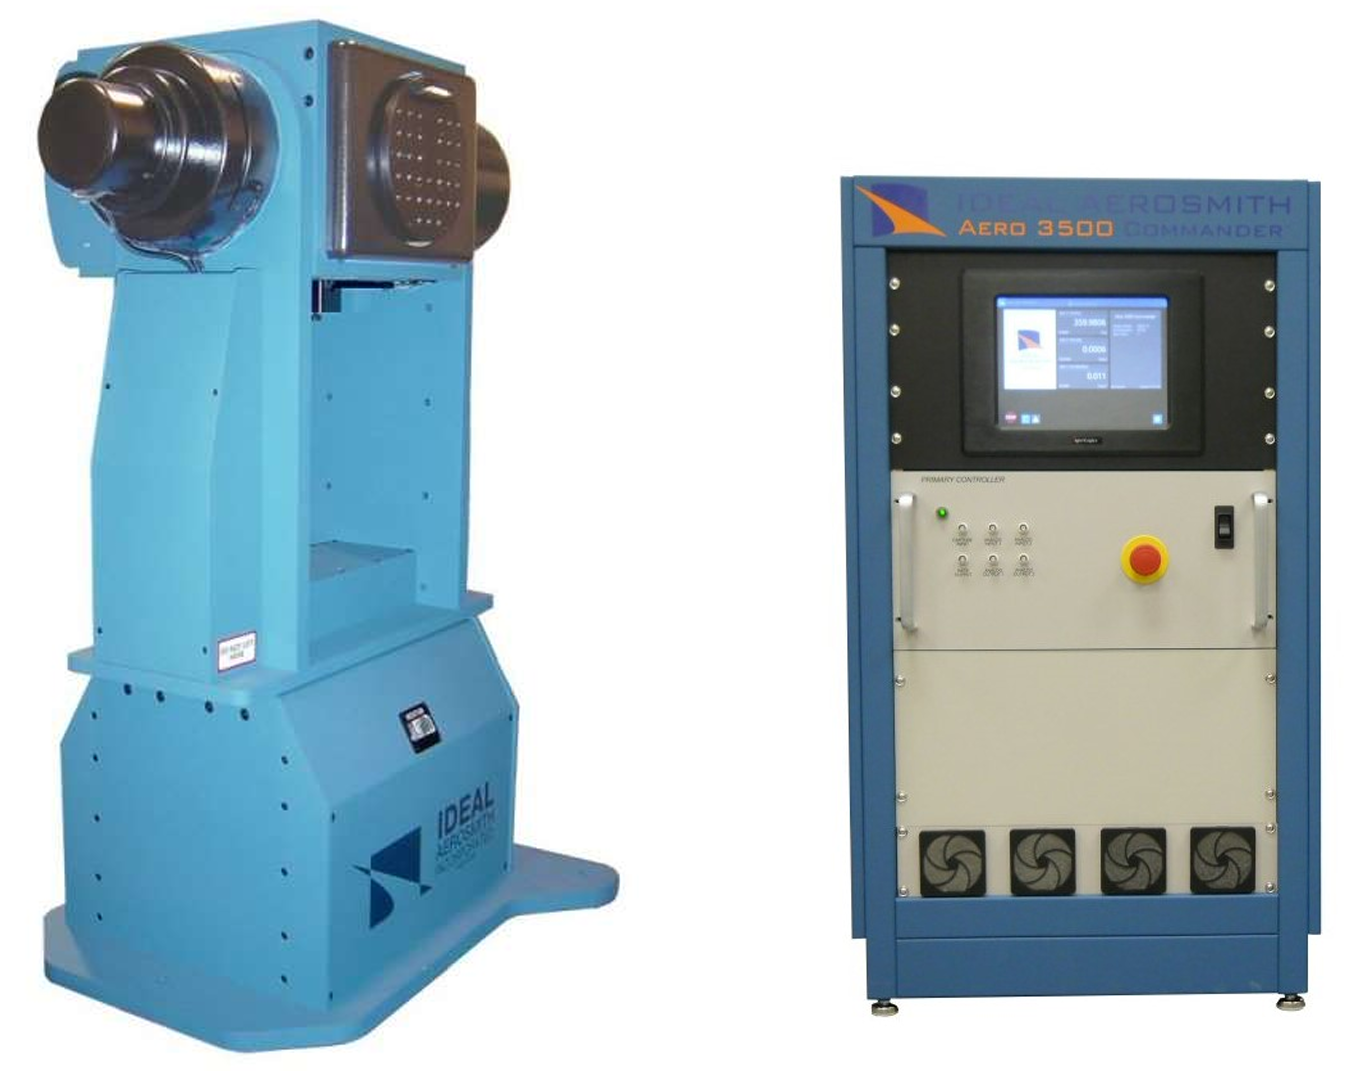
\includegraphics[width=0.65\textwidth]{./images/three_axis_rate_table_example.png}
	\caption{2103C Series Three Axis Position and Rate Table System}
	\label{fig: three axis rate table example}
\end{figure}
\FloatBarrier

Traditional calibration comprises of twelve tests with six for the accelerometers and six for the gyroscopes. In each test, the IMU is stationary for accelerometer tests and spinning at a constant speed for gyroscope tests. Each test is completed for a set amount of time, usually 60 seconds, and the measurements are averaged. Table \ref{tab: traditional_calibration_tests} lists the six tests as well as the quantity for each averaged test result.

\begin{table}[h!]
	\centering
	\begin{tabular}{|p{7cm}|p{7cm}|}
		\hline
		\textbf{Accelerometer Tests} & \textbf{Gyroscope Tests} \\ \hline
		\begin{itemize}
			\item Point X-Axis Up $\left(\bar{\bv{f}}^{\,+\textrm{x}}\right)$
			\item Point X-Axis Down $\left(\bar{\bv{f}}^{\,-\textrm{x}}\right)$
			\item Point Y-Axis Up $\left(\bar{\bv{f}}^{\,+\textrm{y}}\right)$
			\item Point Y-Axis Down $\left(\bar{\bv{f}}^{\,-\textrm{y}}\right)$
			\item Point Z-Axis Up $\left(\bar{\bv{f}}^{\,+\textrm{z}}\right)$
			\item Point Z-Axis Down $\left(\bar{\bv{f}}^{\,-\textrm{z}}\right)$
		\end{itemize}
		&
		\begin{itemize}
			\item Positive Spin about X-Axis $\left(\bar{\bv{\omega}}^{\,+\textrm{x}}\right)$
			\item Negative Spin about X-Axis $\left(\bar{\bv{\omega}}^{\,-\textrm{x}}\right)$
			\item Positive Spin about Y-Axis $\left(\bar{\bv{\omega}}^{\,+\textrm{y}}\right)$
			\item Negative Spin about Y-Axis $\left(\bar{\bv{\omega}}^{\,-\textrm{y}}\right)$
			\item Positive Spin about Z-Axis $\left(\bar{\bv{\omega}}^{\,+\textrm{z}}\right)$
			\item Negative Spin about Z-Axis $\left(\bar{\bv{\omega}}^{\,-\textrm{z}}\right)$
		\end{itemize} \\ \hline
	\end{tabular}
	\caption{Traditional IMU Calibration Tests}
	\label{tab: traditional_calibration_tests}
\end{table}
\FloatBarrier

As an example from equation \ref{eq: expanded IMU forward error model}, the accelerometer bias $\bv{b}_a$ can be solved from the collected test data.

\begin{align} 
	\bv{b}_a = \begin{bmatrix} b_{a,x} \\ \\ b_{a,y} \\ \\ b_{a,z} \end{bmatrix} = \frac{1}{2} \begin{bmatrix}
		\bar{f}^{\,+\textrm{x}}_{x} + \bar{f}^{\,-\textrm{x}}_{x} \\
		\\
		\bar{f}^{\,+\textrm{y}}_{y} + \bar{f}^{\,-\textrm{y}}_{y} \\
		\\
		\bar{f}^{\,+\textrm{z}}_{z} + \bar{f}^{\,-\textrm{z}}_{z}
	\end{bmatrix}
\end{align}

All model in parameters in equation \ref{eq: expanded IMU forward error model} can be solved in a similar manner, which have all been listed in section \ref{sec: traditional imu calibration post-processing}.


\subsection{Beyond Traditional IMU Calibration}

While traditional calibration methods have proven successful over the past several decades, there is a push within the navigation community to move to systematic calibration methods \cite{s16060940}. It is difficult to estimate more model parameters with the same limited dynamics, and the piece-meal approach to post-processing IMU calibration data is cumbersome and complicated. Additionally, traditional means of calibration do not provide any sort of measure of uncertainty which many navigation algorithms, i.e., Kalman filters, require for any sort of state estimation.

Therefore, this paper aims to investigate systematic IMU calibration through the lens of inverse problem techniques. \textcolor{red}{Come back here and tell everyone what you ended up doing.}

